\section{Motivation}
\begin{frame}{Structural Attacks}{Invariant Subspaces}
    \begin{block}{Invariant Subspaces~\cite{C:GAAZ11} (Last Year's FSE)}
        Let $U$ be a subspace of $\F_2^n$, and $F : \F_2^n \to \F_2^n$.
        We write $U + a \through{F} U + b$, if
        \begin{equation*}
            \exists a : \exists b : F(U + a) = U + b
        \end{equation*}
    \end{block}
    \begin{block}{Main Idea}
    \begin{center}
        \begin{tikzpicture}[scale=0.8]
            \tikzstyle{every node}=[transform shape];

            \node (left1-space) [draw,rectangle,thick,rounded corners,minimum width=3cm,minimum height=4cm] at (-8,0) {%
                \begin{tikzpicture}[scale=0.7]
                    \node (u) [draw,rectangle,thick, fill=gray!20] {%
                        \begin{tikzpicture}[scale=1.2]
                            \draw[rounded corners=2pt]
                                (-1.2,1.9) -- (-1,1.9) -- (-0.9,1.7) -- (-1.1,1.2) -- (-1,0.9) -- (-1.4,0.6) -- (-1.1,0.1) -- (-1.2,-0.4) -- (-1.5,-0.2) -- (-1.8,-0.3) -- (-2.2,-0.6) -- (-2.7,-0.3) -- (-2.2,0.8) -- (-2.4,1) -- (-2.6,1) -- (-2.7,1.2) -- (-2.6,1.8) -- (-2.3,1.8) -- (-2.1,2.2) -- (-1.6,2.3) -- (-1.4,2.3) -- (-1.4,2.1) -- (-1.3,2) -- (-1.2,1.9);
                        \end{tikzpicture}
                    };
                \end{tikzpicture}
            };

            \node (right1-space) [draw,rectangle,thick,rounded corners,minimum width=3cm,minimum height=4cm] at (-4,0) {%
                \begin{tikzpicture}[scale=0.7]
                    \node (u) [draw,rectangle,thick] {%
                        \begin{tikzpicture}[scale=1.2]
                            \draw[rounded corners=2pt, fill=gray!20]
                                (-1.2,1.9) -- (-1,1.9) -- (-0.9,1.7) -- (-1.1,1.2) -- (-1,0.9) -- (-1.4,0.6) -- (-1.1,0.1) -- (-1.2,-0.4) -- (-1.5,-0.2) -- (-1.8,-0.3) -- (-2.2,-0.6) -- (-2.7,-0.3) -- (-2.2,0.8) -- (-2.4,1) -- (-2.6,1) -- (-2.7,1.2) -- (-2.6,1.8) -- (-2.3,1.8) -- (-2.1,2.2) -- (-1.6,2.3) -- (-1.4,2.3) -- (-1.4,2.1) -- (-1.3,2) -- (-1.2,1.9);
                        \end{tikzpicture}
                    };
                \end{tikzpicture}
            };

            \draw[-latex] (-8,0.5) to [bend left] node[above]{$F$} (-4,0.5);
            \draw[-latex] (-4,-0.5) to [bend left] node[below]{$F^{-1}$} (-8,-0.5);
        \end{tikzpicture}
    \end{center}
    \end{block}
\end{frame}

\begin{frame}{Structural Attacks}{Subspace Trail Cryptanalysis}
    \begin{block}{Subspace Trail Cryptanalysis~\cite{ToSC:GraRecRon16} (Last Year's FSE)}
        Let $U$, $V$ be subspaces of $\F_2^n$, and $F : \F_2^n \to \F_2^n$.
        We write $U \through{F} V$, if
        \begin{equation*}
            \forall a : \exists b : F(U + a) \subseteq V + b
        \end{equation*}
    \end{block}
    \begin{block}{Main Idea}
    \begin{center}
        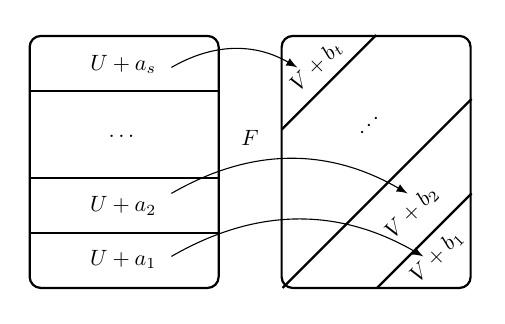
\begin{tikzpicture}[scale=0.8]
            \tikzstyle{every node}=[transform shape];

            \node (left2-space) [draw,rectangle,thick,rounded corners,minimum width=3cm,minimum height=4cm] at (1,0) {};
            \draw[thick] (left2-space.west)+(0,1.125cm) -- node[above, yshift=1.5mm] {$U + a_s$} +(3cm,1.125cm);
            \draw[thick] (left2-space.west)+(0,-0.25cm) -- node[above, yshift=5mm] {\dots} +(3cm,-0.25cm);
            \draw[thick] (left2-space.west)+(0,-1.125cm) -- node[above, yshift=1.5mm] {$U + a_2$}
                                                            node[below, yshift=-1.5mm] {$U + a_1$} +(3cm,-1.125cm);

            \node (right2-space) [draw,rectangle,thick,rounded corners,minimum width=3cm,minimum height=4cm] at (5,0) {};
            \draw[thick] (right2-space.north) -- node[above, yshift=0.5mm, rotate=45] {$V + b_t$} +(-1.5cm,-1.5cm);
            \draw[thick] (right2-space.east)+(0,1cm) -- node[above, yshift=10mm, rotate=45] {\dots} +(-3cm,-2cm);
            \draw[thick] (right2-space.east)+(0,-5mm) -- node[above, yshift=2.5mm, rotate=45] {$V + b_2$}
                                                        node[below, yshift=-0.5mm, rotate=45] {$V + b_1$} +(-1.5cm,-2cm);

            \node (right-f) at (3,0.375) {$F$};

            \draw[-latex] (1.75,-0.5) to [bend left] (5.5,-0.5);
            \draw[-latex] (1.75,-1.5) to [bend left] (5.75,-1.5);
            \draw[-latex] (1.75,+1.5) to [bend left] (3.75,+1.5);
        \end{tikzpicture}
    \end{center}
    \end{block}
\end{frame}

\begin{frame}{The Problem}{How to search efficiently for subspace trails?}
    \begin{block}{Can't we just activate a single S-box and check to what this leads us?}
        \begin{center}
            The short answer is:\\No!\footnote{The long answer is this talk.}
        \end{center}
    \end{block}
\end{frame}

\begin{frame}{Outline}{}
    \begin{block}{Outline}
        \vspace{0.5em}
        \tableofcontents
    \end{block}
\end{frame}

\begin{frame}{Preliminaries, Notations}
    \begin{block}{Subspace Complement}
        If $U$ is a subspace of $\F_2^n$, we denote by $U^\perp$ it's \emph{complement}:
        \vspace{-0.5em}
        \begin{equation*}
            U^\perp \coloneqq \set{u \in \F_2^n \given \forall x \in U: \angles{x, u} = 0}
            \vspace*{-0.5em}
        \end{equation*}
    \end{block}
    \begin{block}{Derivative}
        Let $F : \F_2^n \to \F_2^n$.
        We denote the \emph{derivative of $F$ in direction $u$} by
        \vspace*{-0.5em}
        \begin{equation*}
            \Delta_u(F)(x) \coloneqq F(x) + F(x + u)
            \vspace*{-0.5em}
        \end{equation*}
    \end{block}
    \begin{block}{Linear Structure}
        Let $F : \F_2^n \to \F_2^n$.
        Then $(\alpha, u)$ is called a \emph{linear structure}, if
        \vspace*{-0.5em}
        \begin{equation*}
            \exists c \in \F_2 : \forall x \in \F_2^n : \angles{\alpha, \Delta_u(F)(x)} = c
            \vspace*{-0.5em}
        \end{equation*}
    \end{block}
\end{frame}

\section{Intuition}
\begin{frame}{Intuition}{The Image of the Derivative is in the Subspace}
    \begin{block}{Observation}
        Let $U \through{F} V$, then for every $u \in U$:
        \begin{align*}
            x \in U + x &\through{F} F(x) \in V + b \\
            x+u \in U + x &\through{F} F(x+u) \in V + b
        \end{align*}
        implying $F(x) + F(x + u) \in V$.
    \end{block}
\end{frame}

\section{Algorithm}
